% Theorie: Physikalische Grundlagen von Versuch/Messverfahren, Gleichungen ohne Herleitung knapp erklären
\section{Theorie}
\label{sec:theorie}

Im Folgenden wird bla bla

\subsection{Begriffe der Austrittsarbeit und die Energieverteilung der Leitungselektronen}
\label{sec:Begriffe der Austrittsarbeit und die Energieverteilung der Leitungselektronen}

Eine große Anzahl der Metalle sind kristalline Festkörper, welche ausgezeichnete elektrische Leitfähigkeit besitzen.
Diese Tatsache lässt sich damit erklären, dass die Atome, welche auf den kristallgitterplätzen sitzen, komplett ionisiert sind.
Somit bilden die Inonen ein periodisches Gitter, welches von freigesetzten Elektronen eingehüllt ist.
Diese Elektronen befinden sich im Kraftfeld sämtlicher Inonen und werden als Leitungselektronen bezeoichnet.
Das Gitterpotential ist eine vom Ort abhängige periodische Funktion. Diese nimmt an den Gitterpunkten einen hohen positiven Wert an, weiter 
entfernt von den Punkten ist der Wert des Gitterpotentials nur wenig veränderlich. Somit lässt sich durch eine
Näherung sagen, dass das Gitterpotential konstant ist. Zusammenfassendkann gesagt werden, dass im Metallinnere ein konstantes 
positvives Potential, welches um $\phi$ verschieden zum Außenraum ist, herrscht. Die Elektronen können sich daher 
frei bewegen und demnach die elektrische Leitfähigkeit erzeugen.

Wenn ein Elektron das Metallinnere verlassen will, muss dieses die Austrittsarbeit zu dem gegeben Potential $\xi$ leisten.
In \autoref{fig:potentialtopf} wird dies anhand des Poetentialtopf-Modells gezeigt.
% hier abbildung nutzen
\begin{figure}[H]
    \centering
    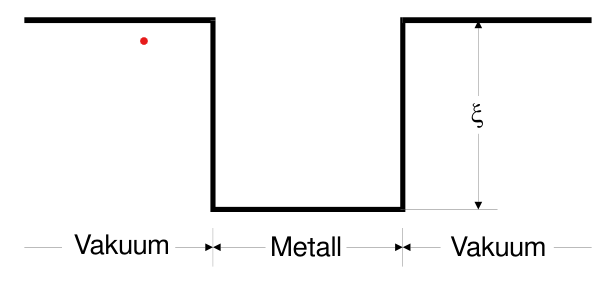
\includegraphics[width=0.5\linewidth]{content/grafik/potential.png}
    \caption{Darstellung des Potentialtopf-Modells eines Metalls.\cite{elektron}}
    \label{fig:potentialtopf}
\end{figure}

Die Quantentheorie beantwortet die Frage, ob das Elektron die benötigte Energie aufbringen kann.
Elektronen können ausschließlich diskrete Energiewerte annehmen. Das Elekron hat einen habzahligen Spin und 
unterliegt demnach dem Pauli-Verbot. Dieses besagt, dass jeder mögliche Zustand mit der vorausgesetzten Energie $E$ nur von zwei
Elektronen eingenommen werden kann, wenn diese entgegengesetzten Spin haben. Somit besitzen die Elektronen auch am Nullpunkt
eine endlich Energie. Diese ist abhängig von den Elektronen pro Volumeneinheit im Metall. Der Begriff für diese Energie bei $T = 0$
wird Fermische Grenzenergie $\zeta $ genannt. Für Zimmertemperatur gilt für alle Metalle $\zeta \gg \symup{k}\symup{T}$.
Durch die Fermi-Dirscsche Verteilungs Funktion 
\begin{equation}
    f(E)= \frac{1}{\exp{\frac{E -\zeta}{\symup{k}\symup{T}}}+1} ,
    \label{eqn:fermi-dis}
\end{equation}
wird die Wahrscheinlichkeit angegeben, dass im thermischen Gleichgewicht der Zustand
mit der Energie $E$ erreicht ist.
Der Verlauf des Graphen der Fermi-Diracschen Verteilungsfunktion ist in \autoref{fig:fermi} zu sehen.

\begin{figure}[H]
    \centering
    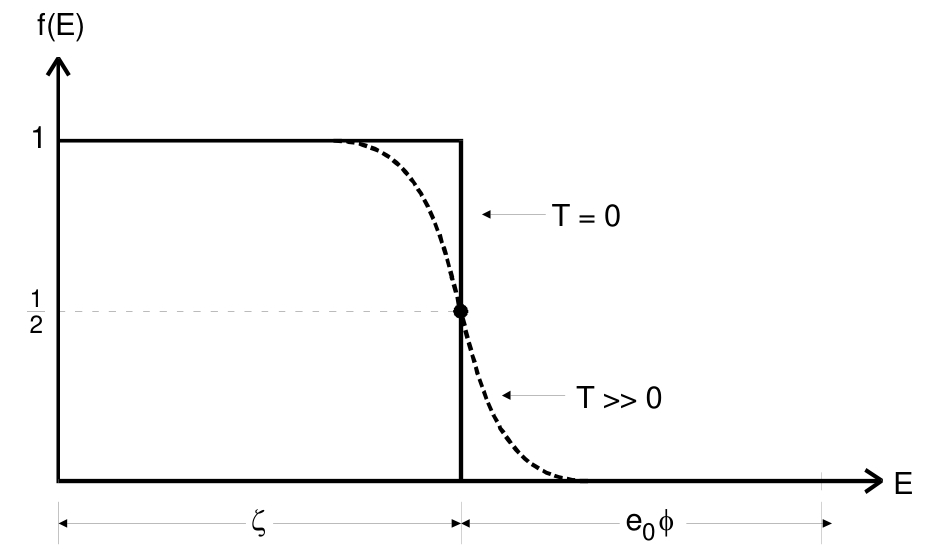
\includegraphics[width=0.5\linewidth]{content/grafik/fermi.png}
    \caption{Der Verlauf der Fermi-Diracschen Verteilungsfunktion am absoluten Nullpunkt.\cite{elektron}}
    \label{fig:fermi}
\end{figure}

Es kann abgelesen werden, dass ein Eletron mindestens eine Energie von $\zeta + e_0 \phi$ vorweisen muss, damit 
es die Metalloberfläche verlassen kann. Für den Fall,dass das gegebenen Metall Wolfram ist, kann eine
Näherung getroffen werden
\begin{equation}
    f(E) \approx \exp{\frac{E -\zeta}{\symup{k}\symup{T}}} .
\label{eqn:naehrung}
\end{equation}

\subsection{Berechnung der Sättigungsstromdichte bei der thermischen Elektonenemission}
\label{sec:Berechnung der Sättigungsstromdichte bei der thermischen Elektonenemission}

Mithilde der \autoref{eqn:naehrung} lässt sich die Sättigungsstromdichte in Abhängigkeit zur Temperatur errechnen.
Schlussendlich folgt für für die Sättigungsstromdichte $j_S(T)$ die Richardson-Gleichungen
\begin{equation}
    j_S(T) = 4\symup{\pi} \frac{e_0\cdot m_0 \cdot \symup{k}^2}{h^3} \symup{T}^3 \exp{\frac{-e_0 \phi}{\symup{k}\symup{T}}}.
\end{equation}

\subsection{Die Hochvakuum-Diode}
\label{sec:Die Hochvakuum-Diode}

Um den Sättigungsstrom einer emittierenden Metalloberfläche zu messen, muss ein Hochvakuum vorliegen, da sonst die
Elektronen mit den Gasmolekülen wechselwirken würden. Weiter wird ein elektrisches Feld benötigt, welches die ausgetretenden Elektronen
absaugt. Diese dafür vorgesehene Apperatur heißt Hochvakuum-Diode. Die Schaltskizze einer solchen Apperatir ist in \autoref{fig:diode} 
dargestellt.

\begin{figure}[H]
    \centering
    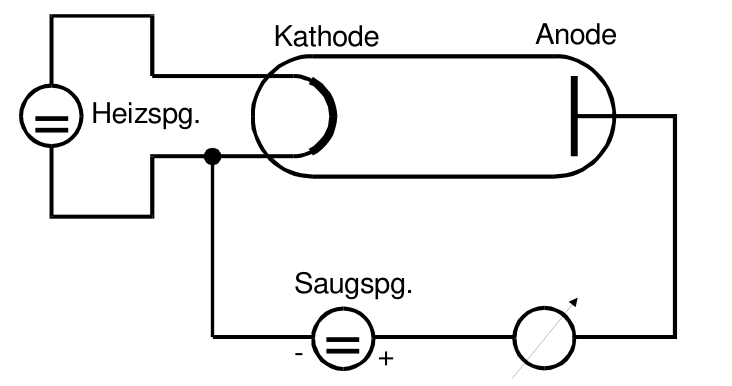
\includegraphics[width=0.5\linewidth]{content/grafik/diode.png}
    \caption{Die grundlegende Schaltskizze einer Hochvakuum-Diode.\cite{elektron}}
    \label{fig:diode}
\end{figure}

\subsection{Die Langmuir-Schottkysche Raumladungsgleichung}
\label{sec:Die Langmuir-Schottkysche Raumladungsgleichung}

Die Geschwindigkeit der Elektronen ist nicht konstant, das führt dazu, dass die Elektronen
eine beschleunigte Bewegung in Richtung auf die Anode ausüben. Dementspechend ist die Raumladungsdichte $\rho$
der Elektronen eine Funktion des Ortes, welche zur Anode hin abnimmt.  Diese Tatsache lässt sich aus der Kontinuitätsgleichung, dass $j$ überall konstant ist,
ableiten.
Die Stromdichte ist gegeben durch
\begin{equation}
    j = - \rho v .
\label{eqn:konti}
\end{equation}
Die Raumladungsdichte $\rho$ beeinflusst daher den Verlauf der Feldstärke zwischen Anode und Kathode.
Sie schirmt das Feld von der Kathode ab. Die emittierten Elektronen werden dann nicht mehr alle von dem
Anodenfeld erfasst. Darauf folgt, dass der zu messene Kathodenstrom kleiner als der zu erwartende Sättigungsstrom.
In der \autoref{eqn:poisson} ist der Zusammenhang der Anodenspannungs - und stroms in der Poissongleichung dargestellt
\begin{equation}
    \increment V = - \frac{1}{\xi_0}\rho .
    \label{eqn:poisson}
\end{equation} 
Angenommen wird, dass die Anode und Kathode unendlich ausgedehnte ebenen Oberflächen sind, welche
mit einem Abstand $a$ zueinander ausgerichtet sind.
Zusammen aus \autoref{eqn:konti} und \autoref{eqn:poisson} folgt der Zusammenhang
zwischen der Stromdichte $j$ und der Anodenspannung $V$
\begin{equation}
    j = \frac{4}{9} \xi_0 \sqrt{2 e_0/m_0} \frac{V^{\frac{3}{2}}}{a^2} ,
\label{eqn:langmuir}
\end{equation}
welcher als Langmuir-Schottkysche Raumladungsgesetz bezeichnet wird. Der Gültigkeitsbereich 
in einem $j$-$V$-Diagramm einer Hochvakuum-Diode wird als Raumladungsgebiet benannt.

In \autoref{fig:raumladung} ist die Ortsabhängigkeit der Potentials, der Feldstärke und der Ladungsdichte im Raumladungsgebiet
eine Hochvakuumdiodenkennlinie aufgetragen.

\begin{figure}[H]
    \centering
    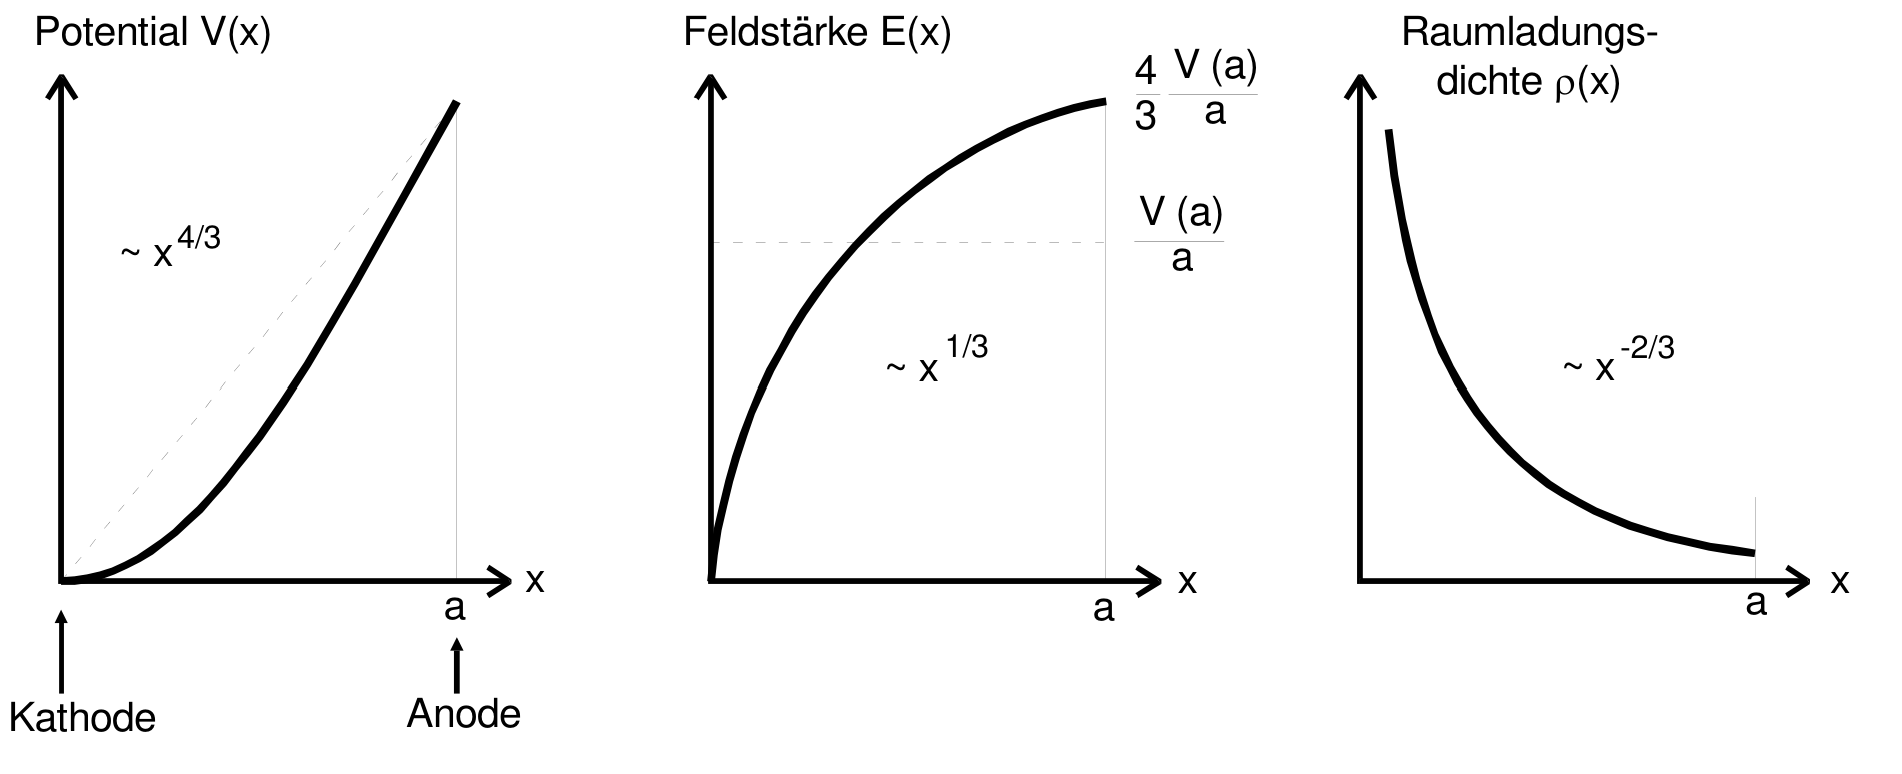
\includegraphics[width=0.5\linewidth]{content/grafik/raumladung.png}
    \caption{Die Darstellung der Ortsabhängigkeit des Potentials $V$, der Feldstärke $E$ und der Ladungsdichte $\rho$ im
    Raumladungsgebiet einer Hochvakuumdiodenkennlinie.\cite{elektron}}
    \label{fig:raumladung}
\end{figure}

\subsection{Das Anlaufstromgebite einer Hochvakuum-Diode}
\label{sec:Das Anlaufstromgebite einer Hochvakuum-Diode}

Aus \autoref{eqn:langmuir} kann abgelesen werden, dass für $j = 0$ auch $V = 0$ gilt.
Durch die Eigengeschwindigkeit, die die Elektronen bei Verlassen der Kathode haben, kann bei $V = 0$
ein geringer Anodenstrom gemessen werden. Für $T > 0$ existieren endlich vile Elektronen, deren Energie größer ist 
als die Austrittsarbeit. Diese Energie 
\begin{equation}
    \increment E = E - \left(\Xi + e_0\phi\right),
\end{equation}    
ist dann die kinetische Energie der Elektronen. Dieser Strom wird als Anlaufstrom bezeichnet.
Das Energieverhältnis im Anlaufstromgebiet ist in \autoref{fig:anlauf} dargestellt.

\begin{figure}[H]
    \centering
    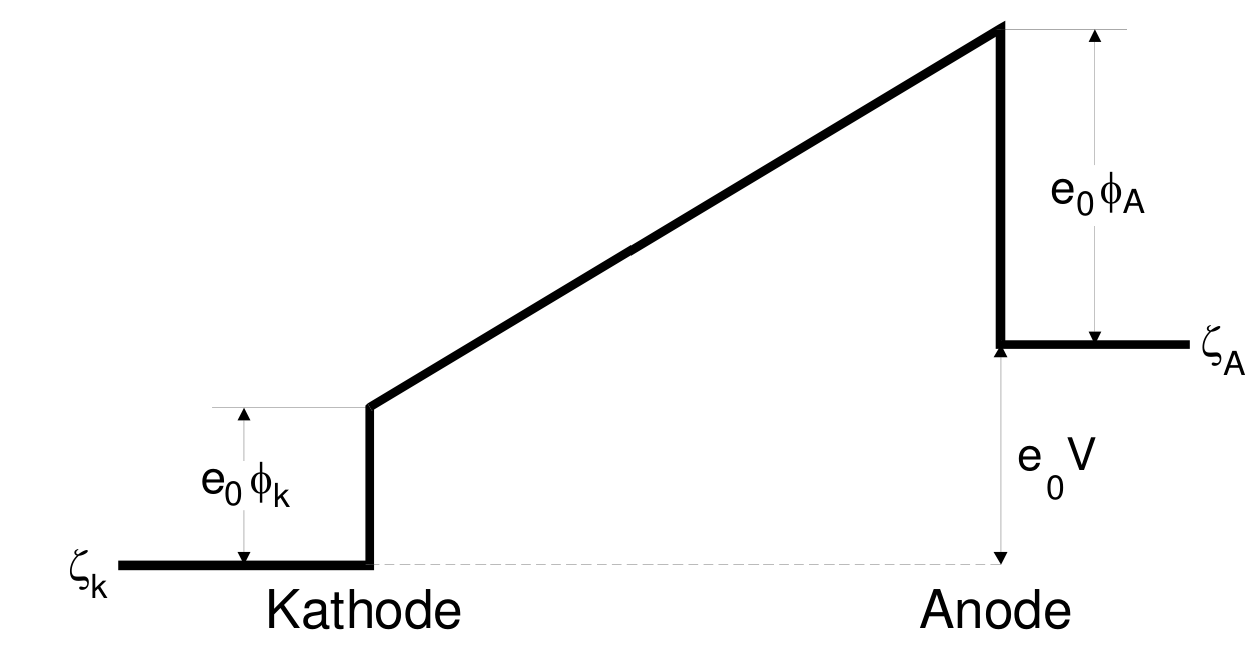
\includegraphics[width=0.5\linewidth]{content/grafik/anlauf.png}
    \caption{Die Potentialverhältnisse in einer Hochvakuum-Diode im Bereich ihres Anlaufstromgebietes.\cite{elektron}}
    \label{fig:anlauf}
\end{figure}

\subsection{Die Kennlinie der Hochvakuumdiode}
\label{sec:Die Kennlinie der Hochvakuumdiode}

Die Kennlinie beschreibt den Zusammenhang der Stromdichte $j$ beziehungsweise dem Anodenstrom $I_A$ 
und dem außen angelegten Potential.

\begin{figure}[H]
    \centering
    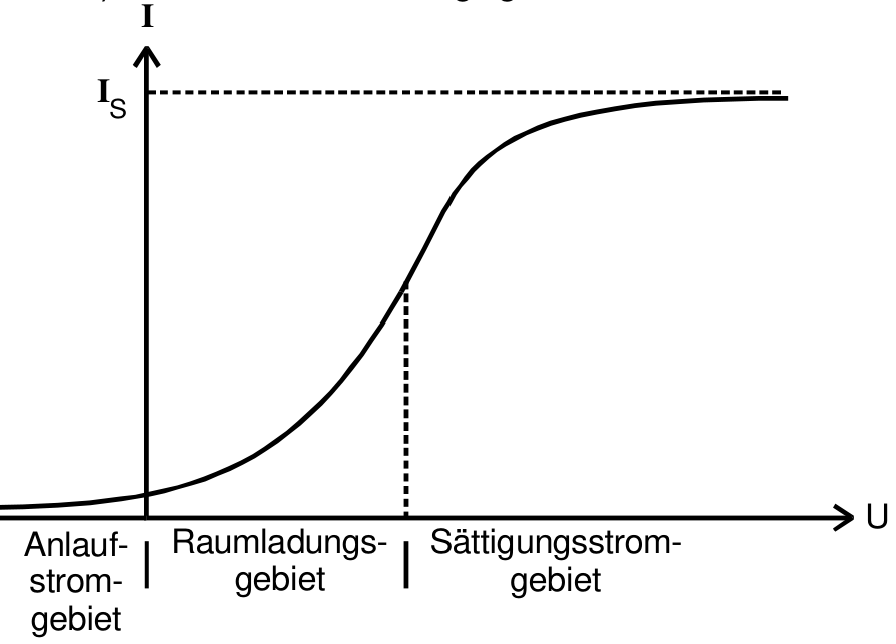
\includegraphics[width=0.5\linewidth]{content/grafik/kennlinie.png}
    \caption{Die Kennlinie einer Hochvakuum-Diode.\cite{elektron}}
    \label{fig:kennlinie}
\end{figure}

Die \autoref{fig:kennlinie} zeigt eine solche Kennlinie einer Hochvakuum-Diode.  Diese lässt sich in drei Abschnitte 
unterteilen: Dem Anlaufstromgebiet, Dem Raumladungsgebiet und dem Sättigungsstromgebiet. Das Anlaufstromgebiet ist durch einen
expoentiellen Anstieg gekennzeichnet, dieses Gebiet liegt im Bereich $V < 0$. Bei dem Raumladungsgebiet  liegt eine $\sqrt{V^3}$- Abhängigkeit vor.
Schlussendlich wird das Raumladungsgebiet lamgsam von dem Sättigungsstromgebite abgelöst. 
Mithilfe dieser Kennlinie kann die Kathodentemperatur und die Austrittsarbeit der Kathode bestimmt werden.